%   MSc Business Analytics Dissertation/Practicum
%
%   Title:     Enhancing Credit Analysis and Assessment using GeoSpatial Techniques
%   Author(s): Deepak Gupta and Shruti Goyal
%
%   This file is the top level file for a dissertation.  It contains:
%   - usepackage commands for any packages required
%   - document-wide parameter settings such as textwidth, etc
%   - The text of small items of the frontmatter (title, abstract, etc.) and backmatter
%
%   Chapter 1: Introduction and basic definitions
%   Chapter 2: Business background and problem
%   Chapter 3: Literature Review
%   Chapter 4: Methodology
%   Chapter 5: Results
%   Chapter 6: Discussion
%   Chapter 7: Conclusions
%
%   Change Control:
%   When     Who   Ver  What
%   -------  ----  ---  --------------------------------------------------------------
%   01Sep10  SMcG  0.0  Developed MSc Business Analytics Dissertation LaTeX template
%   02Sep16  JMcD  0.1  Updated template
%   01Apr17  XX    0.2  Begun dissertation proper
%   02Apr17  YY    0.3  Added ....
%

%% To LaTeX (compile) your whole document, run these \textbf{Response Variable:} DefaultedLoans\\

%% the command line on Linux or Mac OS X but you can run them from inside WinEdt or whatever you use):
%% latex  yourfilename
%% bibtex yourfilename  % NB this is the name of your LaTeX file, not your BibTeX database file!!
%% latex  yourfilename
%% latex  yourfilename
%%
%% Note: you don't need the .tex extension of yourfilename.tex (in fact giving it will confuse bibtex,
%% though latex will understand it).  If you stick with the name thesis.tex for this file, you would use
%% latex thesis etc
%%
%% There are two approaches to where to put the supporting files (LaTeX style (package) files, etc).  Either:
%% 1. Put them all in the same directory as this file (quick and dirty); or
%% 2. Many style (package) files such as natbib.sty, lineno.sty may already be installed on your system, but if
%%    not, just download them e.g., from ctan.org, and copy them to YOURBASEDIRECTORY/texmf/tex/latex
%%    Copy the BibTeX style file mscBA.bst to YOURBASEDIRECTORY/texmf/bibtex/bst
%% Approach 2 will make these files visible to any other LaTeX docs you produce.  Here, YOURBASEDIRECTORY is
%% typically your home directory.

\documentclass[a4paper,12pt,bibtotoc,notitlepage,oneside]{book}
% remove ``oneside'' when printing the final version since that
% will have plenty of blank pages already!

% the bibtotoc may be needed to make your references appear in the Contents, also liststotoc etc

% Preamble

% LaTeX Packages to use
\usepackage{makeidx}
%\usepackage{showidx} % for drafts: shows in margin what will be indexed
\usepackage{amsthm,amsmath,amsfonts,amssymb,latexsym,graphicx,appendix,subfigure}
% the ams* packages provide the (very useful) LaTeX extensions from the AMS (Amer. Math. Soc.)
% latexsym provides some useful extra symbols
% graphicx gives control over image files, e.g., width, etc
% appendix gives more fine-tuned control over the appendices
% subfigure lets you put multiple figures (and tables) in a figure environment, so you can refer to them individually, e.g., Figure~6(b).
\usepackage{algorithm2e} % handles algorithms in a nice way, akin to tables and figures
\usepackage[subfigure]{tocloft}  % package allows you to control the design of table of contents, figures and tables. use subfigure for compatibility -- jmmcd
\usepackage{natbib}   % gives more control over references and style of citation.  Has a lot of options, e.g., can use the [sectionbib] option to have multiple bibliographies in my document, listed in sections rather than chapters. Need this package for Chicago Manual of Style BibTeX referencing and the MScBA derived style
\usepackage{lineno}   % useful for early draft, so a reviewer can list by pageno+lineno where to make changes
% Packages you may like to use
% \usepackage{fancyhdr}  % more control over contents of page headers and footers for documentclass book
% \usepackage{psfrag}  % if using eps files for images, this package lets you replace text in those images, so you can have the same font type and size in both text and images.
% \usepackage{layout} % prints an overview of all the page margins, if you include \layout
%\usepackage[sectionbib]{natbib} if using multiple bibliography files
%\usepackage{chapterbib}
%\usepackage{doublespace} % for double spacing, e.g. initial versions for correcting
%\usepackage[nottoc]{tocbibind} % puts almost everything in the Table of Contents

% include your own macro / declaration files, if any
\usepackage{booktabs}
\usepackage{graphicx}
\usepackage{eurosym}
%   Macros
%   Esp. Theorem styles for amsart/amsbook document classes (currently enabled)
%
%   Sean McGarraghy
%
%   Change Control:
%   Date      Ver  Reason
%   --------  ---  --------------------------------------------------------------
%   12/05/98  0.1  Begun
%

\newcommand*{\Ax}  {Axiom~}
\newcommand*{\Df}  {Definition~}
\newcommand*{\Th}  {Theorem~}
\newcommand*{\Co}  {Corollary~}
\renewcommand*{\Pr}{Proposition~}
\newcommand*{\Lm}  {Lemma~}
\newcommand*{\Rk}  {Remark~}
\newcommand*{\Ex}  {Example~}
\newcommand*{\Exe} {Exercise~}
\newcommand*{\Eq}  {Equation~}
\newcommand*{\dfn} {definition}

\theoremstyle{plain}                 % Default

\newtheorem{thm}{Theorem}[chapter]
\newtheorem{lemma}[thm]{Lemma}
\newtheorem{lem}[thm]{Lemma}
\newtheorem{propn}[thm]{Proposition}
\newtheorem{pr}[thm]{Proposition}
\newtheorem{prp}[thm]{Propn.}
\newtheorem{cor}[thm]{Corollary}
\newtheorem{fact}[thm]{Fact}
\newtheorem{conj}[thm]{Conjecture}
\newtheorem{claim}{Claim}[]

\theoremstyle{definition}

\newtheorem{dm}{}  % Dummy theorem name for numbering only, independent of section
\newtheorem{dmy}[thm]{}  % Dummy theorem name for numbering only
\newtheorem{defn}[thm]{Definition}
\newtheorem{ex}[thm]{Example}
\newtheorem{exe}[thm]{Exercise}

\theoremstyle{remark}

\newtheorem{rmk}[thm]{Remark}
\newtheorem{notn}[thm]{Notation}
\newtheorem{note}[thm]{Note}
\newtheorem{cmt}[thm]{Comment}
\newtheorem{case}[thm]{Case}
\newtheorem{intr1}[thm]{Introduction}
\newtheorem{intro}[thm]{Introduction}

\newenvironment{pf}{\vspace{-4pt}\noindent\begin{proof}}{\end{proof}\vspace{2pt}}




%   General LaTeX Declarations (try -adobe-courier-medium-r-normal--18-180-75-75-m-110-iso8859-2)
%
%   Sean McGarraghy
%
%   Change Control:
%   Date      Ver  Reason
%   --------  ---  --------------------------------------------------------------
%   12/02/98  0.1  Begun
%

% Where to hyphenate words LaTeX doesn't know

\hyphenation{neigh-bour-hood neigh-bour-hoods}
\hyphenation{Bel-field}

% Short commands for italic, bold etc fonts

\newcommand*{\tr}[1]{\textrm{#1}}
\newcommand*{\ti}[1]{\textit{#1}}
\newcommand*{\tb}[1]{\textbf{#1}}
\newcommand*{\ts}[1]{\textsl{#1}}
\newcommand*{\tc}[1]{\textsc{#1}}
\newcommand*{\mr}[1]{\mathrm{#1}}
\newcommand*{\mb}[1]{\mathbf{#1}}
\newcommand*{\tth}[1]{{\slshape #1}}
\newcommand*{\df}[1]{\textbf{#1}}      % put the thing being defined in bold

\newcommand*{\bs}{$\backslash$}
\newcommand*{\ol}[1]{\overline{#1}}
\newcommand*{\cnj}[1]{\overline{#1}}
\newcommand*{\nth}[1]{\ensuremath{{#1}^{\textrm{th}}}}% superscripted `th' for counting
\newcommand*{\nst}[1]{\ensuremath{{#1}^{\textrm{st}}}}% superscripted `st' for counting
\newcommand*{\nnd}[1]{\ensuremath{{#1}^{\textrm{nd}}}}% superscripted `nd' for counting
\newcommand*{\nrd}[1]{\ensuremath{{#1}^{\textrm{rd}}}}% superscripted `rd' for counting

% commonly occurring text in Maths documents

\newcommand*{\eg}  {e.\,g.~}
\newcommand*{\ie}  {i.\,e.~}
\newcommand*{\ff}  {\textrm{if and only if }}
\newcommand*{\A}   {\textrm{ for all }}
\newcommand*{\all} {\textrm{ for all }}
\renewcommand*{\AA}{\ensuremath{\forall~}}
\newcommand*{\E}   {\textrm{ there exists }}
\newcommand*{\EE}  {\ensuremath{\exists~}}
\newcommand*{\st}  {\textrm{ such that }}
\newcommand*{\sta} {\textrm{ such that, for all }}
\newcommand*{\tfae}{the following are equivalent}
\newcommand*{\Tfae}{The following are equivalent}
\newcommand*{\wrt} {with respect to }
\newcommand*{\wolog}{without loss of generality}
\newcommand*{\Wolog}{Without loss of generality}
\newcommand*{\ftsoc}{for the sake of contradiction}
\newcommand*{\resp}{respectively}
\newcommand*{\RHS} {right hand side}
\newcommand*{\LHS} {left hand side}
\newcommand*{\Pf}  {\noindent\tb{Proof: }}            % for backwards compatibility only
\newcommand*{\eop} {~~\vrule height 5 pt width 5 pt depth 0 pt\relax}
\newcommand*{\QED} {\mbox{}\hspace{\fill}\eop}

\newcommand*{\fn}  {function}
\newcommand*{\vsp} {vector space}

\newcommand*{\ind} {independent}
\newcommand*{\dep} {dependent}
\newcommand*{\lcmb}{linear combination}
\newcommand*{\lind}{linearly independent}
\newcommand*{\ldep}{linearly dependent}
\newcommand*{\di}  {dimension}
\newcommand*{\fd}  {finite-dimension}
\newcommand*{\cp}  {characteristic polynomial}
\newcommand*{\de}  {determinant}
\newcommand*{\evl} {eigenvalue}
\newcommand*{\evc} {eigenvector}
\newcommand*{\sle} {system of linear equations}
\newcommand*{\ERO} {elementary row operation}
\newcommand*{\ECO} {elementary column operation}
\newcommand*{\repn}{representation}

\newcommand*{\UCD} {University College Dublin} 

\newcommand*{\itema}[1][a]{\item[(\emph{#1})]} 
\newcommand*{\ita}[1][a]{(\emph{#1})} 

% Math Roman abbreviations e.g. Gal(), Aut() etc.

\newcommand*{\len}{\ensuremath{\operatorname{length}}}% 
\newcommand*{\rank}{\ensuremath{\operatorname{rank}}} % RANK of matrix/linear map
\newcommand*{\nll}{\ensuremath{\operatorname{nullity}}} % NULLity of linear map
\newcommand*{\diag}{\ensuremath{\operatorname{diag}}} % DIAGonal matrix
\newcommand*{\cond}{\ensuremath{\operatorname{cond}}} % CONDition number
\newcommand*{\sign}{\ensuremath{\operatorname{sign}}} % SIGNature
\newcommand*{\sgn} {\ensuremath{\operatorname{sgn}}}  % SiGN of permutation
\newcommand*{\imp}{\ensuremath{\mathbin\Rightarrow}}  % IMPlies sign
\renewcommand*{\Im}{\ensuremath{\operatorname{Im}}}   % IMage (of a map)
\newcommand*{\zv} {\ensuremath{\mathbf{0}}}           % Zero vector
\newcommand*{\zs}[1]{\ensuremath{{#1}^{-1}(0)}}       % Zero Set of function #1
\renewcommand*{\i}[1]{\ensuremath{{#1}^{-1}}}         % Inverse of geezer #1

% spacing/heading commands

\newcommand*{\cpb}{\vspace{\fill}\pagebreak}          % Clean PageBreak inside paragraph
\newcommand*{\cb}{\hspace*{\fill}\\*[\medskipamount]} % Clean Break inside paragraph
\newcommand*{\cbb}{\hspace*{\fill}\\[\medskipamount]} % Clean Break, may have page Break
\newcommand*{\cbs}{\hspace*{\fill}\\*[\smallskipamount]} % Small Clean Creak inside paragraph
\newcommand*{\cbbs}{\hspace*{\fill}\\[\smallskipamount]} % Small Clean Creak, may have page break
\newcommand*{\cbl}{\hspace*{\fill}\\*}                % No gap Clean Break inside paragraph
\newcommand*{\cbbl}{\hspace*{\fill}\\}                % No gap Clean Break, may have page break

\newcommand*{\qt}[1]{\ensuremath{\quad\text{#1}\quad}}
\newcommand*{\qqt}[1]{\ensuremath{\qquad\text{#1}\qquad}}

\newcommand*{\subhead}[1]{  
            \begin{center}
            \tb{#1}
            \end{center}\\*}


% Various inclusion, ideal, equivalence, mapping symbols

%\newcommand*{\squig}{\sim\!\sim\!\rightarrow}  % old definition
\newcommand*{\eqv} {\ensuremath{\mathbin\Leftrightarrow}}  % EQuiValence sign
\newcommand*{\app} {\ensuremath{\rightarrow}}          % APProaches/tends to (limit)
\newcommand*{\map} {\ensuremath{\longrightarrow}}      % set MAPs to (long arrow)
\newcommand*{\tmap}[1]{\ensuremath{
                      \stackrel{\ssk{#1}}{\map} }}    % scriptsize #1 atop ---> arrow
\newcommand*{\mpt}{\ensuremath{\longmapsto}}          % element maps to (long arrow with bar)
\newcommand*{\tmpt}[1]{\ensuremath{
                               \stackrel{#1}{\mpt}}}  % scriptsize #1 atop |--> arrow
\newcommand*{\cng}{\ensuremath{\equiv}}               % CoNGruent to 
\newcommand*{\rel}{\ensuremath{\sim}}                 % single tilde RELation sign
\newcommand*{\nul}{\ensuremath{\emptyset}}            % NULl set 
\newcommand*{\su} {\ensuremath{\subset}}              % SUbset of
\newcommand*{\se} {\ensuremath{\subseteq}}            % Subset of/Equal to
\newcommand*{\sne}{\ensuremath{\subsetneqq}}          % Subset of but Not Equal to
\newcommand*{\sm} {\ensuremath{\smallsetminus}}       % set difference (Set Minus)
\newcommand*{\la} {\ensuremath{\langle}}              % Left Angle bracket
\newcommand*{\ra} {\ensuremath{\rangle}}              % Right Angle bracket
\newcommand*{\du} {\ensuremath{\dot{\cup}}}           % Disjoint Union (dot over cup sign)
\newcommand*{\rt}{\right}
\newcommand*{\lt}{\left}
\newcommand*{\oo}{\ensuremath{\infty}}                % oo = infinity
\newcommand*{\fp}[3]{\ensuremath{{#1}:{#2}\map{#3}}}  % Function/maP f:A--->B
\newcommand*{\ma}[3]{\ensuremath{{#1}:\R^{#2}\map\R^{#3}}} % MAp f:R^n--->R^m
\newcommand*{\lma}[4][]{linear map{#1} \ma{#2}{#3}{#4}} % linear map(s) f:R^n--->R^m
\newcommand*{\cpd}[1][A]{\ensuremath{\det({#1}-\l I)}} % char poly eg det(A-lI)

% Logic and proof
\newcommand*{\LT} {\texttt{T}}
\newcommand*{\LF} {\texttt{F}}
\newcommand*{\NOT}{\mathop\mathrm{not}}
\newcommand*{\AND}{\mathbin\mathrm{and}}
\newcommand*{\OR} {\mathbin\mathrm{or}}

% Binomial coefficient
\newcommand*{\bin}[2]{\ensuremath{\binom{#1}{#2}}}

% Binomial coefficient (textstyle i.e. Small font)
\newcommand*{\sbin}[2]{\ensuremath{\tbinom{#1}{#2}}}

% Binomial coefficient (displaystyle i.e. Big font)
\newcommand*{\bbin}[2]{\ensuremath{\dbinom{#1}{#2}}}

% derivatives
\newcommand*{\dd}[1]{\ensuremath{\displaystyle{\frac{d}{d{#1}}}}}

\newcommand*{\polyn}[3][n]{\ensuremath{{#3}_0+{#3}_1{#2}+\cdots+{#3}_{#1}{#2}^{#1}}}

% MATRICES

% two commonly used building blocks for matrices

% identity matrix
\newcommand*{\idmat}{\ensuremath{ 
1      & 0      & \cdots & 0       \\
0      & 1      & \cdots & 0       \\
\vdots & \vdots & \ddots & \vdots  \\
0      & 0      & \cdots & 1          } }

% matrix consisting of zeros
\newcommand*{\zeromat}{\ensuremath{ 
0      & 0      & \cdots & 0       \\
\vdots & \vdots & \ddots & \vdots  \\
0      & 0      & \cdots & 0          } }

% matrix consisting of asterisks
\newcommand*{\astmat}{\ensuremath{ 
*      & *      & \cdots & *       \\
\vdots & \vdots & \ddots & \vdots  \\
*      & *      & \cdots & *          } }

% Greek letters - abbreviations

\renewcommand*{\a}{\ensuremath{\alpha}}
\renewcommand*{\b}{\ensuremath{\beta}}
\newcommand*{\g}{\ensuremath{\gamma}}
\renewcommand*{\d}{\ensuremath{\delta}}
\newcommand*{\e}{\ensuremath{\varepsilon}}
\newcommand*{\z}{\ensuremath{\zeta}}
\newcommand*{\h}{\ensuremath{\eta}}
\renewcommand*{\th}{\ensuremath{\vartheta}}
%\newcommand*{\io}{\ensuremath{\iota}}
\renewcommand*{\k}{\ensuremath{\kappa}}
\renewcommand*{\l}{\ensuremath{\lambda}}
\newcommand*{\m}{\ensuremath{\mu}}
\newcommand*{\n}{\ensuremath{\nu}}
\renewcommand*{\r}{\ensuremath{\rho}}
\newcommand*{\s}{\ensuremath{\sigma}}
\renewcommand*{\t}{\ensuremath{\tau}}
\renewcommand*{\u}{\ensuremath{\upsilon}}
\newcommand*{\f}{\ensuremath{\varphi}}
\renewcommand*{\c}{\ensuremath{\chi}}
\newcommand*{\x}{\ensuremath{\xi}}
\newcommand*{\p}{\ensuremath{\psi}}
\renewcommand*{\o}{\ensuremath{\omega}}

\newcommand*{\G}{\ensuremath{\Gamma}}
\newcommand*{\D}{\ensuremath{\Delta}}
\newcommand*{\T}{\ensuremath{\Vartheta}}
\renewcommand*{\L}{\ensuremath{\Lambda}}
\renewcommand*{\L}{\ensuremath{{\textstyle{\bigwedge}}}}
%\newcommand*{\Si}{\ensuremath{\Sigma}}
\newcommand*{\U}{\ensuremath{\Upsilon}}
\newcommand*{\F}{\ensuremath{\Phi}}
\renewcommand*{\P}{\ensuremath{\Psi}}
\renewcommand*{\O}{\ensuremath{\Omega}}


% Math mode blackboard and calligraphic (script) letters

\newcommand*{\N}{\ensuremath{\mathbb{N}}}
\newcommand*{\Z}{\ensuremath{\mathbb{Z}}}
\newcommand*{\Q}{\ensuremath{\mathbb{Q}}}
\newcommand*{\R}{\ensuremath{\mathbb{R}}}
\newcommand*{\C}{\ensuremath{\mathbb{C}}}
\renewcommand*{\H}{\ensuremath{\mathbb{H}}}
\newcommand*{\FF}{\ensuremath{\mathbb{F}}}

\newcommand*{\sA}{\ensuremath{\mathcal{A}}}
\newcommand*{\sB}{\ensuremath{\mathcal{B}}}
\newcommand*{\sC}{\ensuremath{\mathcal{C}}}
\newcommand*{\sD}{\ensuremath{\mathcal{D}}}
\newcommand*{\sE}{\ensuremath{\mathcal{E}}}
\newcommand*{\sF}{\ensuremath{\mathcal{F}}}
\newcommand*{\sG}{\ensuremath{\mathcal{G}}}
\newcommand*{\sH}{\ensuremath{\mathcal{H}}}
\newcommand*{\sI}{\ensuremath{\mathcal{I}}}
\newcommand*{\sJ}{\ensuremath{\mathcal{J}}}
\newcommand*{\sK}{\ensuremath{\mathcal{K}}}
\newcommand*{\sL}{\ensuremath{\mathcal{L}}}
\newcommand*{\sM}{\ensuremath{\mathcal{M}}}
\newcommand*{\sN}{\ensuremath{\mathcal{N}}}
\newcommand*{\sO}{\ensuremath{\mathcal{O}}}
\newcommand*{\sP}{\ensuremath{\mathcal{P}}}
\newcommand*{\sQ}{\ensuremath{\mathcal{Q}}}
\newcommand*{\sR}{\ensuremath{\mathcal{R}}}
\newcommand*{\sS}{\ensuremath{\mathcal{S}}}
\newcommand*{\sT}{\ensuremath{\mathcal{T}}}
\newcommand*{\sU}{\ensuremath{\mathcal{U}}}
\newcommand*{\sV}{\ensuremath{\mathcal{V}}}
\newcommand*{\sW}{\ensuremath{\mathcal{W}}}
\newcommand*{\sX}{\ensuremath{\mathcal{X}}}
\newcommand*{\sY}{\ensuremath{\mathcal{Y}}}
\newcommand*{\sZ}{\ensuremath{\mathcal{Z}}}


\linespread{1.25}         % spacing between lines
\parindent0pt             % no paragraph indentation
\parskip\smallskipamount  % small space between paragraphs

%\setlength{ \topmargin      }{  -1cm }
%\setlength{ \textheight     }{  24cm }
\setlength{ \textwidth      }{  14cm }
\setlength{ \oddsidemargin  }{ 1.0cm }
\setlength{ \evensidemargin }{ 1.0cm }

\numberwithin{equation}{section}  % alter this if desired
\numberwithin{figure}{chapter}    % alter this if desired

\pagestyle{plain} % just puts a page number at the bottom of each page
% If you comment out the last line's \pagestyle command, you can control the page headers as follows:
%\def\leftmark{\textsc{YourText1}}  % text to appear in header of left-hand (even numbered) pages, e.g., Chapter Title
%\def\rightmark{\textsc{YourText2}}  % text to appear in header of right-hand (odd numbered) pages, e.g., Thesis Title
%\def\leftmark{\textsc{}}  % gives empty header on left-hand (even numbered) pages
%\def\rightmark{\textsc{}}  % gives empty header on right-hand (odd numbered) pages

% If, in the output, if you find the width of numbers in the Contents, List of Figures, etc is too great
% (e.g. too close to the heading names) uncomment the following
%\setlength{\cftfignumwidth}{3em} % this allows you to control width of numbering in List of Figures
                                 % 4em, 5em etc would be even wider; you can also hardcode 2cm or similar
                                 % but units of em (width of a capital M) or ex (height of a small x) are
                                 % preferred since they vary with the font type / size used

% comment this out for your final version (where you don't want line numbers)
%\linenumbers

\makeindex % generates the index entries (unsorted: need to run makeindex from the command line to sort them)


% Use the following to only include certain chapters (it will speed up compilation of the part you
% are currently working on, should the dissertation as a whole take excessively long to compile).
\includeonly{%
preface%
,
ch1%
,%
ch2%
,%
ch3
,%
ch4%
,
ch5%
,
ch6%
,
ch7%
,
appendix1%
,
appendix2%
,
glossary%
,
notation
}


%% Lay out your thesis as follows (standard book form: some of these are optional):

%% \begin{enumerate}
%% \item Front matter (preliminaries: roman page numbering, i, ii, iii, iv,\ldots)
%%   \begin{enumerate}
%%   \itema{} Title Page, giving (on separate lines, in this order):
%%     \begin{enumerate}
%%     \itema[i] Title
%%     \itema[ii] Author(s), listing previous degree(s), e.g.,\ Joe Bloggs, B.E.
%%     \itema[iii] A thesis submitted to \UCD\ in part fulfilment of the requirements of the degree of
%%           M.Sc.~in Business Analytics
%%     \itema[iv] Michael Smurfit Graduate School of Business
%%     \itema[v] Date (\emph{Month, Year}, e.g.,\ \emph{September, 2010})
%%     \itema[vi] Supervisor(s): Xxx Xxxxx (and Yyy Yyyyy)
%%     \itema[vii] Head of School: Professor Ciar\'an O'h\'Ogartaigh
%%  \end{enumerate}
%%   \itema[b] Dedication
%%   \itema[c] Table of Contents
%%   \itema[d] List of Figures (Illustrations)
%%   \itema[e] List of Tables
%%   \itema[f] List of Algorithms (if any)
%%   \itema[g] Foreword (if any: may precede table of contents)
%%   \itema[h] Preface (including authors' signatures: may precede table of contents)
%%   \itema[j] Acknowledgements (including permissions and other credits)
%%   \itema[k] Abstract
%%   \itema[l] List of important abbreviations (including special fonts, e.g.,\ {\tt fixed width} for program code)
%%  \end{enumerate}
%% \item Body or ``Main Matter'' (the text: arabic page numbering, 1, 2, 3,\ldots)
%%   \begin{enumerate}
%%   \itema{} Chapters of your dissertation, including, but not limited to:
%%     \begin{enumerate}
%% \itema[i] Introduction
%% \itema[ii] Literature Review
%% \itema[iii] Methodology
%% \itema[iv] Results
%% \itema[v] Analysis/Discussion
%% \itema[vi] Conclusions
%%    \end{enumerate}
%%   \itema[b] Epilogue (if any)
%%   \itema[c] Afterword (if any)
%%   \end{enumerate}
%% \item Back matter (loose ends: continue arabic page numbering)
%%   \begin{enumerate}
%%   \itema{} Appendices (if any: may include program code if not too long)
%%   \itema[b] Endnotes
%%   \itema[c] Glossary of terms
%%   \itema[d] Bibliography (References)
%%   \itema[e] List of contributors
%%   \itema[f] Notation Index / List of Symbols
%%   \itema[g] Index
%% \end{enumerate}
%% \end{enumerate}


\begin{document}

\frontmatter % This is the material before chapter 1, page numbering in Roman numerals ii, iii, iv, ...

\title%[Abbreviated Title for Header]
    {\bf Enhancing Credit Analysis and Assessment using Geo Spatial Techniques\\}

\author{Deepak Kumar Gupta, B.Tech. Computer Science \\ Shruti Goyal, B.Tech. Instrumentation and Control}  % change to suit!
\date{}
\maketitle % this outputs the title using the \title and \author above

{\normalsize
\vfill
\begin{center}
% Alternative for PhD
%\textup{A thesis submitted to University College Dublin in part fulfilment
%of the requirements of the degree of Philosophi\ae~Doctor}
\textup{A Practicum submitted to University College Dublin in part fulfilment
of the requirements of the degree of M.Sc.~in Business Analytics}
\end{center}
\vfill
\begin{center}
Michael Smurfit Graduate School of Business,
University College Dublin
\end{center}
\vfill
\begin{center}
\textit{September, 2017}
\end{center}
\vfill
\begin{center}
\textup{Supervisors: Dr. Peter Keenan, UCD \\ Selwyn Hearns, KPMG IRM Audit}
\end{center}
\vfill
\begin{center}
\textup{Head of School: Professor Ciar\'an \'O h\'Ogartaigh}
\end{center}
\vfill
}

\thispagestyle{empty} % it is conventional to have no page number on the title page (page i)

\clearpage % inserts a page break


% Subsequent distinct parts of the document begin with a \chapter*{} command: this produces a chapter with
% no number.  Note that in a book or amsbook document class, each chapter starts on a new odd-numbered page.


%% Dedication
\chapter*{Dedication}
To our freinds and family for their support and encouragement.


%% Table of Contents
% If you would like the word ``Chapter '' to appear before the chapter number in your Contents, uncomment:
% \renewcommand{\cftchapfont}{Chapter }

\cleardoublepage
\tableofcontents
%\renewcommand{\cftchapfont}{}

% Note: to show subfigures, subtables (if any) in the appropriate list below, uncomment the following command
% \setcounter{lofdepth}{2}

% If you find your Table and/or Figure captions are taking up too much space in the Lists below, use the
% following in the appropriate Table and Figure environments in your chapters:
%\caption[Short Caption]{An Excessively Long and Descriptive Caption, which is probably too long in any case\ldots}
% Then the short caption appears in the list, while the long one appears in the text under your Table/Figure.

% below, the \addcontentsline{toc}{section}{List of figures} etc ensures these lists appear in the contents

% similarly to the \renewcommand{\cftchapfont}{Chapter } above, you can have the words Table or Figure appear
% in front of every entry in the appropriate list by uncommenting as approapriate:
%\renewcommand{\cftfigfont}{Figure }
%\renewcommand{\cfttabfont}{Table }

\clearpage

%% List of Figures (Illustrations)
\listoffigures\addcontentsline{toc}{chapter}{List of figures}

\clearpage
%% List of Tables
\listoftables\addcontentsline{toc}{chapter}{List of tables}

%% List of Algorithms (if any): need to \usepackage{algorithm2e} for nice algorithm layout and this command
%\listofabbreviations\addcontentsline{toc}{chapter}{List of abbreviations}

%% modify titles with
%% \renewcommand{\cftXtitlefont}{\Huge\itshape}
%% Replace the X with either “toc”, “lof” or “lot” and use any font size you like.
%% Available font sizes are: \tiny, \scriptsize, \footnotesize, \small, \normalsize, \large,
%% \Large, \LARGE, \huge and \Huge.



%% Preface (including authors' signatures: may precede table of contents)
%   MSc Business Analytics Dissertation
%
%   Title:     Aaa Bbbbbbb Cccccccccc
%   Author(s): Xxxxxx Xxxxxxxxx and Yyy Yyyyyyyyy
%
%   Preface
%
%   Change Control:
%   When     Who   Ver  What
%   -------  ----  ---  --------------------------------------------------------------
%   11Feb11  AB    0.1  Begun
%

\chapter*{Preface}

% Some people like to put in a little quote (Knuth in particular loves this)

\begin{quote}
\noindent\textit{Men occasionally stumble over the truth, but most of them pick themselves up and
hurry off as if nothing had happened.}

\hspace{2cm}--- Winston Churchill
\end{quote}

<<<<<<< HEAD
Much of the front matter is optional. In particular, include things like a Dedication, List of Figures, List of Tables, List of Algorithms, only if there are enough of them to justify it and it would help the reader.

Don't include both a Foreword and a Preface since they perform similar roles.

The same goes for appendices, index, glossary, list of notation and terms at the end. Include if they would help the reader.

But always, of course, include the Bibliography.
=======
The basis for this practicum stemmed from our passion towards data exploration, pattern finding, and development of new solutions. Data visualization has always been of our interest. Hence, this practicum presents an interactive visualization. It is our passion to develop interactive dashboards and serves profound insights to all types of users. We could not have achieved the success of our practicum without the constant help and support from our academic supervisor Dr. Peter Keenan and business supervisor Mr. Selwyn Hearns. We faced challenges while doing the research, but doing aggressive investigation has helped us to find answers to our questions. Research of this practicum has given us an opportunity to broaden our knowledge area towards data analysis and optimization of problems.\\

Chapter \ref{C.intro} will provide an overview of the problem this practicum is going to address with brief outline of each chapter.\\

Chapter 2 will discuss the business we are working with and what are the main contributions.\\

In chapter 3 detailed review of academic contributions towards the problem areas can be found. It will explain technologies that have been used in the past and are currently in use. Comparison between traditional systems and advanced methods can be of interest for the readers.\\

Chapter 4 will describe detailed steps of the methods followed while working on this practicum such as implementation, data discovery, etc.\\

Chapter 5 will presents results of the experiments that have been performed during the whole course of the completion of this practicum.\\

Data analysis and patterns that we have found are explained in chapter 6 and chapter 7 will provide closing statements and the scope of improvements in future.\\

The whole process could not have been achieved without a supporting group. At first, our family, who have always encouraged us with love and second, our supervisors, who have been so patient and provided their guidance throughout the practicum process. Thank you our support system for constant support.
>>>>>>> 1a1516efb322395fdc40cc383e296dc5c3686ae8

\vspace{2em}

University College Dublin \hfill Xxxxx Xxxxxxx \\
\today \hfill Yyy Yyyyyyyyy



%% Acknowledgements (including permissions and other credits).  Modify as appropriate

\chapter*{Acknowledgements}
We would like to express our thankfulness to Dr Peter Keenan and Dr James McDermott for constant support and providing answers all our queries related to this work.\\

We also like to thank KPMG, Ireland for sponsoring this project. Mr Selwyn Hearnes, Partner and Mr James Fitzpatrick from KPMG IRM Audit team for their valuable knowledge and support for carrying out this research work.


%% Abstract

%\begin{abstract}
\chapter*{Abstract/Executive Summary}

%%   List of important abbreviations (including special fonts, e.g.,\ {\tt fixed width} for program code)

% Bulk of thesis. line numbers in arabic numerals, 1, 2, 3, ...
\mainmatter

\linespread{1.3} % adjust line spacing (if desired)

% \include all your chapters.  This automatically puts the material on a new page.  Recall that \chapter{} and
% \chapter*{} start a new chapter on a new odd-numbered page, but won't put extra empty pages along with \include
%   MSc Business Analytics Dissertation
%
%   Title:     Aaa Bbbbbbb Cccccccccc
%   Author(s): Xxxxxx Xxxxxxxxx and Yyy Yyyyyyyyy
%
%   Chapter 1: Introduction and basic definitions
%
%   Change Control:
%   When     Who   Ver  What
%   -------  ----  ---  --------------------------------------------------------------
%   11Feb11  AB    0.1  Begun
%

\chapter{Introduction}\label{C.intro}
One of the key activities of banking and financial institutions that enhance their quality and financial system, correct handling, and management of liabilities. The performance of those tasks is very crucial for country's economic development, that Irish government witnessed as Irish property bubble that happened in Celtic Tiger period (late 1990 - 2007). While assessing credit risk, it is essential to validate the accuracy and reliability of credit scores or credit rating for all participants. So, How do banks identify a default event: 1. Nonrepayment of the debt to the bank, 2. Repayment is due for more than 90days.\\

This work will discuss predictive models for enhancement in credit analysis and assessment of residential mortgages registered in Ireland using geospatial locations. There have been many studies and researches on how to assess and analyze credit scoring or credit risk, but very few studies are present that describes assessment using geospatial data. This project will demonstrate how geospatial techniques can be used to enhance further credit analyses that empowers banks and financial institutions to take the much better decision on an application. This project will present predictive model that predicts probability of default and an interactive visualization highly focused on geospatial locations of residences registered in Ireland and bank's branch locations. The purpose of this visualization is to support decision maker to take a more effective decision whether to provide loan on a particular house mortgage or not with the use of predicted probability of default. Models for Credit analysis are developed with the use of decision trees using CART algorithm and logistic regression for binary response (dependent) variables. While building models, potential variables were selected based on Information Value statistics. Credibility and quality of the models were evaluated using approaches such as GINI statistics, prediction accuracy, and ROC (Receiver Operating Characteristic) curve.\\

Credit assessment and analysis plays a crucial role in determining financial strength of businesses and risk estimation that are associated with credit. Following are the main purposes of assessment of credit:
\begin{enumerate}
\item Helps keeping track of the economy (macro economic perception) 
\item Analyses and ensures stability of financial market (macro prudential perspective)
\item Assessment of quality of collateral/mortgage (monetary policy)
\end{enumerate}

\section{Assumptions \& Challenges}

KPMG provided made up data due to conidentiality agreement with their client. Data is generated from pre deined formulas that made data look like original real life data but it could not cover all possible real life scenarios. For example - Data only considers that an applicant will default if it has credit rating of 5 but data did not consider the scenario that an applicant may default if he\/she has a credit rating of 2,3,4 and even 1 in some cases. This depicts a constraint of given data over real life data.\\

Below is a list of assumptions undertaken during the process of practicum:
\begin{enumerate}
\item Property prices have been considered as provided in the data by KPMG, there is no consideration of any time frame. For example, date when property valuation was done. 
\item Geospatial data such as address latitude and address longitude is assumed to be correctly depicts geospatial location a property.
\item A property is considered as a whole, number of apartments and number of floors are ignored. Latitude and longitude of a house consists of 2 floors is same.
\item Dimensions of house and size of the house(number of rooms, bathrooms, lawn, etc) are not considered during model development.
\item This project only focuses on residential properties not on commercial properties. 
\item This project did not consider factors such as neighbourhood, amneties and demographics which affects the property price in the market. However, factors such as location, average price have been considered for predicting probability of default.
\end{enumerate}

\section{Outline}
Below is the flow of the practicum which will give brief description of each chapter:
\begin{itemize}
\item Business Background \\ This chapter describes business need and contributions in detail. It wil explain how this project will contribute towards banks and financial institutions businesses. 
\item Literature Review \\ Chapter 3 presents in-depth study of academic contributions made towards field of credit analysis, geospatial techniques and data visualisation. This chapter will explain in detail what is credit scoring and what techniques have been used in past to enhance assessment of credit. It will show comparison between traditional systems and credi scoring along with algorithms to build model for predicting probability of default. Later, it will describe geospatial techniques and data visualisation technqiues.
\item Methodology \\ Chapter 4 will give detailed explaination of steps and tools that have been used to successfully conduct this project and how different tools have been integrated together.
\item Results \\ Chapter 5 explains the output generated from the methods and algorithms described in the above mentioned chapters. It will describe the graphs and images that hold utermost importance and are relevant to the business need alongwith Tableau dashboards.
\item Discussion \\ This chapter will discuss data limitations and practicality of the models developed that correctly answers business questions. 
\item Conclusion and Future Work \\ This chapter will conclude the outcome of the practicum along with the improvements and future scope of the project.
\end{itemize}

%   MSc Business Analytics Dissertation
%
%   Title:     Aaa Bbbbbbb Cccccccccc
%   Author(s): Xxxxxx Xxxxxxxxx and Yyy Yyyyyyyyy
%
%   Chapter 2: Business Background
%
%   Change Control:
%   When     Who   Ver  What
%   -------  ----  ---  --------------------------------------------------------------
%   11Feb11  AB    0.1  Begun 
%

\chapter{Business Background}\label{C.Business.Background}

\section{Introduction}\label{S.intro2}
KPMG is one of the most renowned Big Four auditors and provides tax, audit, advisory and consultancy services to various clients. Information Risk Management is the service line of the organization that provides information systems security assurance while minimizing risks and frauds. For accuracy of financial reports, IT organizations depend on an effective audit. KPMG's IRM audit team works with clients and auditors to assist them to obtain their desired results; by assuring customers how IT functions are efficiently controlled and by ensuring auditors that their work is efficient and accurate within the guidelines. IRM audit team supports audit planning process and fraud risk assessment to monitor IT risks; supervises processes for a particular industry; supports auditors; assesses application controls design; supports testing phase of the whole audit process. Benefits of the services provided by IRM audit team are efficient and effective audits, impactful audit decisions and opinions, precise identification of business risks and issues reporting to senior management and audit committee.\\

There has been a rapid loan growth since last few decades, that led to aggressive lending(weak controls and lenient standards). This increased lending can come from a volatile source. Auditing loan portfolios is imperative to make sure safety and compliance with regulatory requirements. 
The goal of auditing is to catch errors before the examiners find them and initiate corrective action. This session will help identify what the examiners are looking for in residential real estate, consumer, and commercial loan files regarding both compliance and safety and soundness.\\

with signicant increases in installment credit, singlefamily mortgages, auto enhnancing, and credit card debt. Credit scoring models have been widely used by the financial industry during this time to improve cash flow and credit collectionsThe advantages of credit scoring include reducing the cost of credit analysis, enabling faster credit decisions, closer monitoring of existing accounts, and prioritizing collections
 
%   MSc Business Analytics Dissertation
%
%   Title:     Aaa Bbbbbbb Cccccccccc
%   Author(s): Xxxxxx Xxxxxxxxx and Yyy Yyyyyyyyy
%
%   Chapter 3: Literature Review
%
%   Change Control:
%   When     Who   Ver  What
%   -------  ----  ---  --------------------------------------------------------------
%   11Feb11  AB    0.1  Begun 
%

\chapter{Literature Review}\label{C.LitReview}
\section{Introduction}\label{S.intro3}

In recent years, purchasing capability of an \textbf{economy} has increased due to improvement in their finances, and employment levels. Ranging from buying small household items to\textbf{ expensive items such as a house, a car or an office}. To buy a house or a car, one needs to have a large amount of money available to him; that is not necessarily possible most of the time. \\

\textbf{Start with an exmaple to explain what is loan}. There are certain critical circumstances that can occur anytime, where one may need a certain amount of cash. So one may need to borrow a generous amount of money from some other entity which is called a loan. A loan is lending a sum of money from one entity to another that involves repayment of the amount in near future. Lent amount is called principal amount and amount to be repaid is a summation of principal amount and an interest amount or other charges. It is not as easy as it sounds like, there are certain terms need to be agreed upon by each entity before exchange of the money. A loan can be for an amount taken at one time or can be taken in instalments {Partial Payments]. A loan can be provided by banks, corporations and financial institutions. Banks and financial institutions provide various types of loans as per the need of an applicant, such as personal loans, home loans, business loans, credit card loans and cash advances. There are times when the borrowing amount is very large and banks cannot provide the loan based on verbal agreement, they need to ensure that if an applicant is not able to repay the loan then they need to have a source to recover the lent amount. So, in this case, an applicant needs to apply for a mortgage with the bank.\\

A mortgage or collateral is an instrument that applicant has to pay back with predefined series of payments to the bank and financial institutions. Over a duration of time, an applicant needs to repay the loan inclusive of interest amount in order to free his/her mortgage. In case, if an applicant is not able to repay the loan within predetermined time, then the bank can recover their money by selling or putting it for auction the mortgage. The most common type of mortgage is residential mortgages were applicant gives his/her house to banks and in a case of no repayment then a bank will claim the house to recover the balance amount of the loan. This will give a bank a security that their lent amount is not at risk and over the years they will get back their lent money one way or the other. Mortgages come in various different forms. Most commonly used mortgage types are Fixed Rate Mortgage where applicant repays the loan amount on a fixed rate throughout the period determined and Adjustable Rate Mortgage where interest rate varies as per the changes in market interest rates. Our work is based on analysis of residential mortgages with varied interest types which will be discussed in later sections.\\

Put \textbf{Photo of loan application process folw chart}

Before analysing data based on residential mortgages, one needs to understand the process of giving a loan. Depending upon the requirement an applicant applies for a loan by filling an application form with all the necessary details required by the bank. Bank officials then analyse the application and may ask an applicant for additional information; after evaluation, bank approves or disapproves the loan. Next, borrower and bank sign an agreement that states all the terms and conditions of the loan including determined interest rate and type of mortgage. Lastly, loan amount will disburse and borrower will start repaying the instalments that constitute principal amount and interest amount for predetermined period of time.\\

And, the major question is how do banks decide whether to give a loan or not? This question is of major concern as bank's cash flow highly depends on timely repayment of the loan. Every bank does not have the same procedure but majority of the loan review process is same. Following are few characteristics that bank officials will concentrate while evaluating a loan application:
\begin{enumerate}
	\item Credit history of applicant
	\item Loan to Value ratio
	\item Employment history
	\item Character assessment of applicant
	\item Evaluation of collateral
	\item Financial statements such as bank history, cash flow, etc. 
\end{enumerate}

\section{Credit Risk}\label{C.risk}

Used to reduce the burden of bad debt on banks similar to bubble market crisi

\section{Analysis and assessment of credit}\label{tech.crisk}

Importance of assessing credit worthiness has been increased since, the property crash in 2008. Banks and Financial instituions making efforts to enhace tranditional credit scoring mechanisms by incorporating latest technology and tools. Not only avaiablity data about customer but also rapid development in machine learning and analytics providing a foundation stone to banks. \\

Traditional credit scoring process with random selection of good and bad portfolio from creditors file around 50 - 300 \citet{capon1982credit} chartartestics points from loan portfolios to build a essential subset to perform statastical analysis .

\citep{10.2307/2983268}, Mentioned about three commonly used approaches used for selecting characterstics out of avialble data: Expert Knowledge, Stepwise Statstical procedure and evaulating individual characterstics. Subject Matter Expert(SME) \\


An applicant credit score is generated using credit rating system based on various charterstics points. Thereafter credit score is used depending on the usage of system. There are single cut-off and two cut-off stages in deciding application decision. In single cut-off, credit is granted if applicant score is higher than cut-off; otherwise credit is denied. Some instituations incorportae two stage cut-offs, in this system if credit score is higher than upper cut-off then credit is granted straighted and denied if score is lower thant lower cut-off. If score is between upper and lower cut-off then applicant credit history is pulled to calculate further scoring point and added to credit score. If new total score is higher than upper cut-off then credit is granted else denied.\\

Banks and financial instution sets their own cut-off for credit score based on the probablities of each applicant ability to repay or nonpayment of credit amount.\\

Adding flow chart of Evaulation Process and Pricing
\begin{figure}
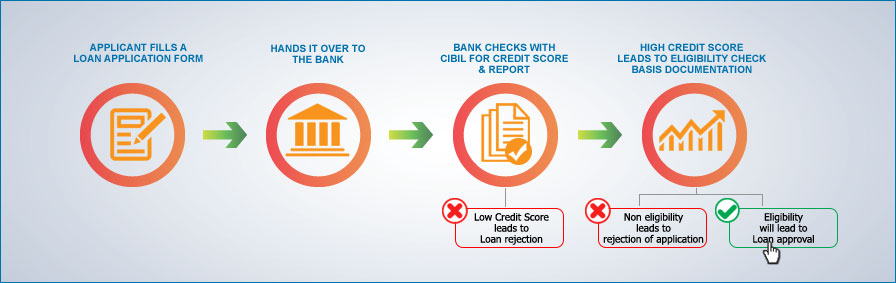
\includegraphics[width=\textwidth]{creditscoreflow.jpg}
\end{figure}

However, Credit Risk has recevied a lot of critisim as well from Academics and Researchers. \citep{al2002credit} has questioned about optimal method to evaulate customers? What are key variables or data points which an analyst must consider while evaulating customer applications? On what basis one can classify an applicant as good or bad?\\


However, apart from above questions following can be useful when building a new credit scoring system. One should evaluate statistical techniques or algorithm by its accuracy to correctly classify historical portfolios into good or bad credit from creditors file. Also, Banks and Financial institution's identified factors that can influence the prediction of credit and loan quality by gathering all possible information from customer applications form, bank transactions history and previous credit history. Credit Analysts analysis of all these information to decide what all variables or characteristics to be included in final the credit model.\\


One of the principal objectives of credit scoring system is to assist Banks and Financial Institutions to streamline their credit management procedure and policy that will enable analysts with an efficient tool which will provide fast and accurate analysis of credit.On the longer run, such tool helps banks to avoid bad credit and scale up bank revenues and profit by selling more financial products to customers.\\


Diffrrerent Technology in Credit Risk:

Linear Regression


\textbf{Discriminant analysis}:

Multiple Discriminat Analysis has been utlized in various research and verticles for variety of applications since its inception by\citep{fisher1936use} 

Durang (1941) was first to use Discriminat analysis for modeling a scoring system that gives prediction about loan repayment. 


Probit analysis


Decision trees

fdgdfh

Expert systems



Neural networks


Genetic programming was introduced by \citet{koza1992evolution} 



























Credit analysis and assessment is very important for banks and financial instituions to evaluate the credit worthiness of an applicant or a borrower. Banks implements various factors while assessing credit risk; such as credit rating, loan to value ratio, probability of default, etc.; that leads to derivation of credit risk rating. Variety of financial techniques have been used by the officials to analyse credit risk. 

\subsection{Examples of citations}\label{SS.citations}

In \citep{Atiyah:1961,Atiyah:1966a,Atiyah:1966b}, Atiyah builds on the work of \citet{Adams:1962} to develop 
the foundations of topological $K$-theory.  \citet{LewMcG:2000} and \citet{McG:2002} later extend parts of 
this to a previously unexplored algebraic setting.

%   MSc Business Analytics Dissertation
%
%   Title:     Aaa Bbbbbbb Cccccccccc
%   Author(s): Xxxxxx Xxxxxxxxx and Yyy Yyyyyyyyy
%
%   Chapter 4: Methodology
%
%   Change Control:
%   When     Who   Ver  What
%   -------  ----  ---  --------------------------------------------------------------
%   11Feb11  AB    0.1  Begun 
%

\chapter{Methodology}\label{C.Methodology}

\section{Overview}\label{S.Ch4.opening}
To assist financial auditor or stakeholder at financial institutions and banks, and to identify such loan portfolio which may default in future based on the geospatial information and financial data. This research work followed the KDD process which involves characteristics variables selection, perform data restructuring, data transformation and data mining for the deployment of a predictive model using visual analytics tools such as Tableau, QlikView, etc.

\textbf{Software \& Tools used:}

Following is the list of tools and softwares that has been used while working on this project:
\begin{description}
  \item[Data Processing:] MS Excel 2017 and Alteryx Desginer 11.0
  \item[Version Control:] Github (github.com)
  \item[Dashboard:] Tableau Professional 10.2 and R Stuio 1.0.36
  \item[Data Storage:] Github Pages (https://pages.github.com/) and Google Drive
\end{description}
\textbf{R Packages used:}
\begin{description}
  \item[Packages required Logisctic Regression Model:] Following packages used to building simple regression and logistic regression based model for predictig the good or bad loan portfolio: glm() with class set to "bionomial" for Logistic Regression and "log" for Poisson regression, ROSE, ROCR, Dplyr, maps, ggplot2
  \item[Decession Tree:] Following r-packages used for building a predictive model based on decision tree: caret, rpart, rattle, ROSE, ROCR, RColorBrewer, party, partykit
\end{description}
\textbf{R Shiny:} R Shiny packages for building interactive dashboards: leaflet, maps, ggmap, gridExtra, htmlwidgets, reshape2. To deploy predictive model on Tableau to build dyanmic and easy to user dashboard R Server used


One may replicate our work on his/her computer having minimum hardware specifications outlined here. This research work carried on following machines. 

% \usepackage{booktabs}
\begin{table}[!htb]
\centering
\caption{System configurations used to carry out this research}
\label{osc4}
\begin{tabular}{|p{3cm}|p{5cm}|p{5cm}|}
\toprule
\textbf{Specification}    & \textbf{System 1 - Lenovo Yoga 500}   & \textbf{System 2 - Dell Inspiron 15} \\ \midrule
\textbf{Operating System} & Windows 10 Professional               & Windows 7 Professional               \\
\textbf{Processor}        & Intel(R) Core(TM) i3-5005CU @ 2.00GHz & Intel(R) Core(TM) i3-3217U @ 1.80GHz \\
\textbf{RAM}              & 4.00 GB                               & 4.00 GB                              \\
\textbf{System Type}      & 64-bit OS, x64-Based Processor        & 32 -bit Operating System             \\ \bottomrule
\end{tabular}
\end{table}


\section{Data Processing \& Analysis}\label{ch4.3}

\subsection{Overview}
One requires the accessibility to the right set of data, and information on which statistical and modelling techniques can be applied to start any data oriented research in analytics domain, KPMG, Ireland provided data set. This data set contains historical data of various loan portfolios that maintained by each branch of banks or financial institutions. Also, this dataset has geospatial information about credit account along with their transactional history of previous loans. Credit scoring model requires being trained with a correct set of characteristics variables to provide the prediction with high accuracy.\\

This project has been carried out in four stages as outlined below:
\begin{itemize}
  \item Data Selection \& Processing
  \item Model Design \& Implementation
  \item Testing \& Model Results
  \item Deployment \& Visualizations
\end{itemize}

\subsection{Data Set}
Dataset format: .xlsx\\
Number of attributes: 35\\
Total number of records: 237,390\\
All the variables and attributes have been carefully studied and analysed to decide what key factors will be used to develop the model. Based on the availability of RAM on the current system, it was decided to build a model on selected characteristics variables. One may train the model with all possible variables as well if system hardware allows. Below is the list of variables in original dataset:

\begin{verbatim}

[1] "ContractRef"           "LoanBalance"    "InterestType"    
[4] "ProbationaryLoans"     "MortgageType"   "NewLoan"         "NIM"  
[8] "DefaultedLoans"        "CreditRating"   "InterestIncome"  "LTV"               
[12] "LTVCategory"          "MortgageYears"  "PropertyValue"             
[15] "MaturityDate"         "BookingDate"    "LastValuationDate"      
[18] "County"               "Branch"         "Address"   
[21] "Town"                 "InArrears"      "AddressLongitude" 
[24] "AddressLatitude"      "DaysInArrears"  "ArrearsCategory"
[27] "HousePriceMovement"   "ValueInArrears" "ValuationAgeYears"
[30] "UpdatedPropertyValue" "LTVUpdated"     "LTVCategoryUpdated"
[33] "CreditRatingMovement" "InterestRate"   "AnnualPYMT"

\end{verbatim}

Below is the comprehensive list of all variables that have been chosen for the model creation:
\begin{description}
  \item[ContractRef]: Unique reference number assigned to each portfolio
  \item[InterestType]: There are three types of interest rate: Fixed, Tracker and Variable
  \item[MortgageType]: Whether property is bought for "buy-to-let" or "owner occpied"
  \item[NewLoan]: Is portfolio is new or existing?
  \item[ProbationaryLoans]: Has loan been taken on probation?
  \item[DefaultedLoans]: Classify if the loan has defaulted in the past
  \item[LTVCategory]: 5 Level categorized pre-assigned to each loan account
  \item[CreditRating]: Each account is rated from 1-5 scale on the basis of credit union policy
  \item[MortgageYears]: How many years mortgage has been taken for?
  \item[CreditRatingMovement]: Percentage that indicates how credit rating has moved from previous value for an application
  \item[LTV]: Ratio of applied loan amount to property evaluation value 
  \item[LoanBalance]: How much loan amount is left to repay?
  \item[InterestIncome]: How much interest amount bank is earning?
  \item[PropertyValue]: Recent property evaluation amount
  \item[AnnualPYMT]: How much amount is getting repaid to the bank by the applicant annually?
  \item[AddressLatitude]: Latitude value of the house on map
  \item[AddressLongitude]: Longiitude value of the house on map
  \item[County]: Name of the county where house is located
  \item[InArrears]: Any amount that has not been paid earlier on time
  \item[ArrearsCategory]: Category that defines duration of Arrears such as more than 90 days
\end{description}

\textbf{Structure of the Data}
\begin{verbatim}
Classes ‘tbl_df’, ‘tbl’ and 'data.frame':	36696 obs. of  20 variables:
 $ ContractRef         : chr  "00000CONTR00111034" "00000CONTR00146183"
    "00000CONTR00175040" "00000CONTR00171901" ...
 $ InterestType        : Factor w/ 3 levels "Fixed","Tracker",..:
    2 3 2 1 2 3 2 2 2 3 ...
 $ MortgageType        : Factor w/ 2 levels "Buy to Let",
     "Owner Occupied": 1 2 2 2 2 2 2 2 2 2 ...
 $ NewLoan             : Factor w/ 2 levels "No","Yes":
    1 1 1 1 1 1 1 1 2 1 ...
 $ ProbationaryLoans   : Factor w/ 2 levels "No","Yes": 
    2 1 1 1 1 1 1 1 1 1 ...
 $ DefaultedLoans      : Factor w/ 2 levels "No","Yes":
    2 2 2 2 2 2 2 2 2 2 ...
 $ LTVCategory         : Factor w/ 11 levels "> 100%","0 to 10%",..:
    11 8 11 5 3 5 9 11 9 9 ...
 $ CreditRating        : Factor w/ 5 levels "1","2","3","4",..:
    4 2 4 4 3 2 3 3 4 2 ...
 $ MortgageYears       : int  31 30 30 29 29 32 28 35 29 31 ...
 $ CreditRatingMovement: int  3 0 0 0 2 -3 0 0 0 0 ...
 $ LTV                 : num  0.983 0.65 0.93 0.368 0.167 ...
 $ LoanBalance         : num [1:36696, 1] -0.647 -0.297 1.418
    -0.986 -1.32 ...
  ..- attr(*, "scaled:center")= num -1.05e-17
  ..- attr(*, "scaled:scale")= num 1
 $ InterestIncome      : num [1:36696, 1] -0.71 -0.132 1.53 
    -0.203 -1.1 ...
  ..- attr(*, "scaled:center")= num -2.14e-17
  ..- attr(*, "scaled:scale")= num 1
 $ PropertyValue       : num [1:36696, 1] -1.3 -0.311 0.779
    -0.511 -0.205 ...
  ..- attr(*, "scaled:center")= num -2.51e-17
  ..- attr(*, "scaled:scale")= num 1
 $ AnnualPYMT          : num [1:36696, 1] -1.2756 -0.2211 
    0.9057 -0.3651 ...
  ..- attr(*, "scaled:center")= num 9.48e-18
  ..- attr(*, "scaled:scale")= num 1
 $ AddressLatitude     : num  52.4 53.3 52.8 53.7 53.4 ...
 $ AddressLongitude    : num  -7.7 -6.27 -6.74 -6.68 -6.21 ...
 $ InArrears           : Factor w/ 2 levels "No","Yes":
    1 1 1 1 1 1 1 2 1 2 ...
 $ County              : Factor w/ 26 levels "Carlow","Cavan",..: 
      22 6 1 17 6 9 16 22 6 6 ...
 $ ArrearsCategory     : chr  "0" "0" "0" "0" ...
\end{verbatim}

\section{Implementation}\label{}

\begin{figure}
\centering
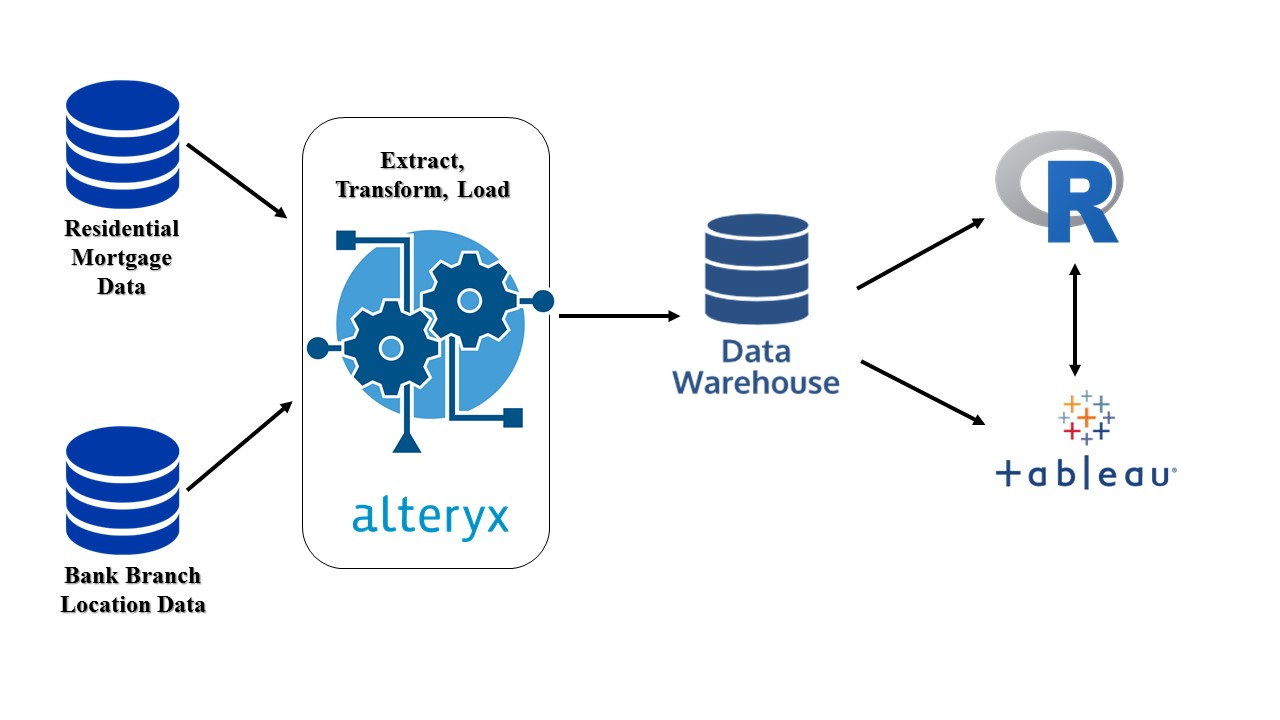
\includegraphics[width=\textwidth]{ETL.jpg}
\caption{ETL \& Data Model Architecture}{\textbf{Source}: Designed using MS Office}
\end{figure}


\subsection{Data Extraction} Prior building predictive model in R one, need to process and analyse the data. The primary objective is to identify any outliers and to normalise the available data set. \cite{sola1997importance}, observed that un-normalized data tends to increase square mean error and then deviate the model prediction. Therefore, it is important to treat data and normalised it's all variables so that model works with high precision and accuracy. One can also do data pre-processing using R as well, but Alteryx provides graphical user interface to select features and settings that makes whole data processing phase easy and fast\\

\textbf{Alteryx Desginer} tool allow one to build workflow to prepare data from multiple data sources on the go and by using features such as 'Select', 'Random Sample', 'Transform' and 'Output' one can easily prepare data for the predictive model \citep{dinsmore2016self}. Alteryx can process large amount of dataset and optimized it to be ready for data modelling in R.

\begin{center}
\begin{figure}[ht]
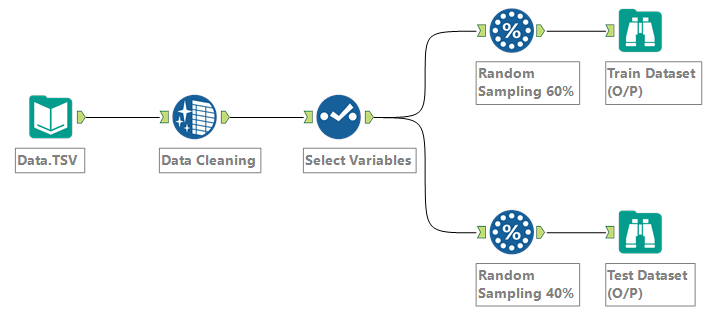
\includegraphics[width=\textwidth]{dataprocess.png}
\centering
\caption{Data Processing using Alteryx}{\textbf{Source:} Designed using in Alteryx Designer v11}
\label{fig:dataprocessing}
\end{figure}
\end{center}

In fig.\ref{fig:dataprocessing}, raw data has been read using \emph{Input tool}, then null values, white spaces etc removed using \emph{Cleansing Tool} and variables selection has been done using \emph{Select Tool}. To create train data set and test data set \emph{Random Sample \% tool}, which allows generating sample datasets.\\

\subsection{Data Transformation}
In Alteryx, there is no provision to normalize data. Processed data from Alteryx is loaded into \textbf{R Studio} for data normalization or scaling using in built functions such as scale($<variable>$) and log($<variable>$) on $LoanBalance$, $PropertyValue$, $InterestIncome$ and $AnnualPYMT$ as these variables are crucial paramters for credit scoring to make unbaised prediction model.\\

\textbf{R Studio}: Data from Alteryx is loaded to R Studio for the development of prediction model. R is used to identify patterns or correlation in variables using \emph{ggplot2}, \emph{plot.ly}, \emph{leaflets}. Two predictive models have developed based Logistic Regression and Decision Tree algorithms and both models performance evaluated concerning accuracy. Trained model is saved on the hard drive and loaded in Tableau, and with the help of R Server, Tableau allows the user to build dynamic visualizations. In Tableau, calculated fields can dynamically invokes R engine to perform calculations and then R results output values back to Tableau, so that visualizations can be designed.\\


\subsection{Data Loading}\label{tableau}
\textbf{Integration of R in Tableau}: Processed and transformed data is loaded into Tableau for building business dashboards. Credit analyst or auditors will use the dashboard to identify locations where the most number of loan default happenings or identify those portfolios which have provided incorrect information, etc. business decisions can be made with the help of credit scoring dashboard.\\

\textbf{Installtion of R Server:} Local instance of R Server is deployed by installing \emph{Rserve} package from R console. To invoke R Server with following command:
      \begin{verbatim}
      install.packages("Rserve")
      library(Rserve)
      Rserve()
      \end{verbatim}

\textbf{Setting in Tableau}:\\

In Tableau, go to \emph{Settings and Performance} under \emph{Help} menu and then select \emph{Manage External Service Connection}. Following settings are required to connect with R server:
      \begin{verbatim}
      Server: "localhost" or "127.0.0.1
      Port: 6311
      \end{verbatim}

R scripts are written in calculated fields of Tableau to make calls to R using in built functions in Tableau such as \emph{SCRIPT\_STR} and \emph{SCRIPT\_REAL}



\section{Predictive Model}

\subsection{Overview}
\cite{shmueli2011predictive}, define predictive analytics as the process of building statistical models using data mining algorithm with an objective to predict the outcome on future data set. A model is evaluated based on its predictive power or accuracy. As discussed in section \ref{c3.tech}, Logistic regression and Decision Tree are most commonly algorithms for building predictive models for credit scoring. Based on the requirement of predictive algorithms, data type of certain variables has been converted using below code:

\begin{verbatim}
Datav2$CreditRating <- as.factor(Datav2$CreditRating)
Datav2$InterestType <- as.factor(Datav2$InterestType)
Datav2$MortgageType <- as.factor(Datav2$MortgageType)
Datav2$NewLoan <- as.factor(Datav2$NewLoan)
Datav2$ProbationaryLoans <- as.factor(Datav2$ProbationaryLoans)
Datav2$LTVCategory <- as.factor(Datav2$LTVCategory)
Datav2$InArrears <- as.factor(Datav2$InArrears)
Datav2$County <- as.factor(Datav2$County)
Datav2$DefaultedLoans <- as.factor(Datav2$DefaultedLoans)
Datav2$LoanBalance <- scale(Datav2$LoanBalance)
Datav2$PropertyValue <- scale(Datav2$PropertyValue)
Datav2$InterestIncome <-scale(Datav2$InterestIncome)
Datav2$AnnualPYMT <-scale(Datav2$AnnualPYMT
\end{verbatim}

\subsection{Logistic Regression}

Logistic regression is the most commonly used technique in credit scoring as it works on binary response variables, i.e., 0 or 1 \citep{hilbe2011logistic}. In fig. \ref{fig:logistic}, output results of standard logistics regression function lies between 0 and 1 only. In this research work output of response variable, i.e., the probability of default $p=1$ is considered as 'Yes' and $p=0$ is considered as 'No'. Probability is represented using logistic function (logit) and the probability of binary response variable based on the one, or more independent variables.

\begin{center}
\begin{figure}[ht]
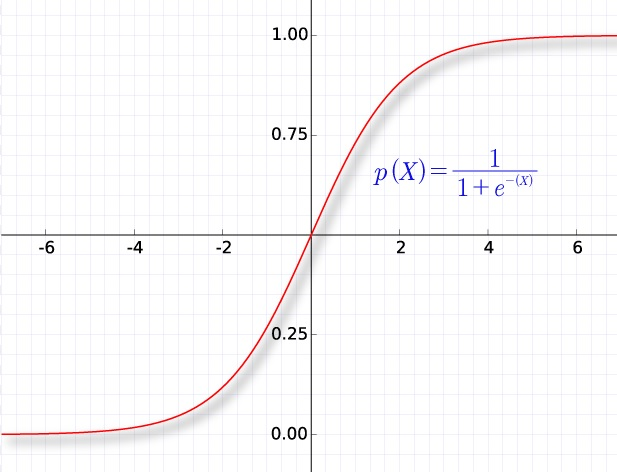
\includegraphics[width=\textwidth]{logistic.jpg}
\centering
\caption{Standard Logistic Regression}{\textbf{Source:} http://www.thefactmachine.com/wp-content/uploads/2015/03/13-Sigmoid.gif}
\label{fig:logistic}
\end{figure}
\end{center}

\subsubsection*{Model Settings:}

\textbf{Response Variable:} DefaultedLoans\\
\textbf{Family (Function):} "Binomial" (Logit)

\subsubsection*{Model Implementation Details:}
Initially, To train the model for all variables available in the dataset, but the model couldn't be trained because R engine failed to allocate 5.0GB vector space for the model. Following the line of code is used:

\begin{verbatim}
library(stats)
m2 <- glm(DefaultedLoans ~., family = "binomial", data = trainDatav2)
\end{verbatim}

<<<<<<< HEAD
=======
Next, model is trained with selective variables set and following code is used:

\begin{verbatim}
simpleglmv2 <- glm(DefaultedLoans ~ CreditRating + InterestIncome + 
    log(PropertyValue) + log(LoanBalance) + AnnualPYMT + LTV + 
    InterestType + NewLoan + ProbationaryLoans + MortgageYears + 
    MortgageType + InArrears + County + AddressLatitude + AddressLongitude, 
    family = "binomial", data = trainDatav2)
\end{verbatim}
>>>>>>> 7f79cd9dd6bc200d97b54f224dc698794bfa066b

Trained model is used to predict output for test dataset using following code:
\begin{verbatim}
testDatav2$prediction <- predict(simpleglmv2, newdata=testDatav2,
type="response")
\end{verbatim}


\subsection{Decission Tree}

As discussed in section \ref{logit}, Decision Trees has two most commonly used algorithm for credit scoring i.e. CART and C4.5. Classification and regression trees (CART) has been implemented using rpart() package available in R to build predicive model. rpart() syntax is \begin{verbatim}
rpart(formula, data=, method=,control=)
\end{verbatim}

\begin{description}
  \item[formula =] DefaultedLoans ~ NewLoan + County + LoanBalance + PropertyValue + InterestIncome + CreditRating + AnnualPYMT + County + LTV + LTVCategory + InArrears + MortgageType + MortgageYears + AddressLatitude + AddressLongitude
  \item[data =]trainDatav2
  \item[method =] "Class"
  \item [control =] Parameters for controlling the growth of tree. \\
  \textbf{control =  rpart.control(minisplit=500,cp = 0.001))} At least 500 observations should be on a node before attempting a split and reduce the split fit factor by 0.001 before being attempted.
\end{description}

Packages such as rattle(), RColorBrewer(), etc. used to enhance the overall decision tree.

\subsubsection*{Model Implementation Details:}

\begin{verbatim}
library(rpart)
library(rattle)					# Fancy tree plot
library(rpart.plot)			# Enhanced tree plots
library(RColorBrewer)		# Color selection for fancy tree plot
library(party)					# Alternative decision tree algorithm
library(partykit)				# Convert rpart object to BinaryTree
library(caret)
defaultLoanTree <- rpart(DefaultedLoans ~ NewLoan + County + LoanBalance 
+ PropertyValue + InterestIncome + CreditRating + AnnualPYMT + County 
+ LTV + LTVCategory + InArrears + MortgageType + MortgageYears 
+ AddressLatitude + AddressLongitude ,method = "class",data=trainDatav2,
control =  rpart.control(minisplit=5,cp = 0.001))

save(fit, file = "Model/classificationTreeV2.rda")
print(defaultLoanTree)
prp(defaultLoanTree)
tree.1 <- defaultLoanTree
fancyRpartPlot(tree.1)
\end{verbatim}

Finally, Model performance of logistic regression and decision tree has been evaulated based on GINI, ROC metrics.

\section{Tableau \& Dashboards} 

Tableau professional software is used to develop the business dashboard that will be utilised by end users such as credit analyst, auditors, banks officials, etc. In Tableau, CSV file connector is used to connect to the data source ( sample dataset); then it is used to prepare various graphs and geospatial dashboard. Calculated field in Tableau allows making the call to R engine directly. By using calculated field options in Tableau, the predictive model is loaded into Tableau to make direct calls to R engine. Instructions and settings mentioned in section \ref{tableau} used as is to connect Tableau with R. \\

In the dashboard, the user can select an origin city or region and distance (in miles) from that origin. Based on these inputs user will be able to take the business decision such as investigating a loan account when property value of a particular house is higher than the area average property value, or opening new branches near by to areas for which a high number of loan applications is coming in. Following calculations are performed in Tableau calculated fields:

\textbf{Calculation for distance from Origin city}:
\begin{verbatim}
3959 * ACOS
(
  SIN(RADIANS(LOOKUP(AVG([Address Latitude]), First()))) * 
  SIN(RADIANS(AVG([Address Latitude]))
) +
  COS(RADIANS(LOOKUP(AVG([Address Latitude]), First()))) * 
  COS(RADIANS(AVG([Address Latitude]))) * 
  COS(RADIANS(AVG([Address Longitude])) - RADIANS(LOOKUP(AVG([Address Longitude]),
  First())))
)
\end{verbatim}


\textbf{Calculation script for logistic regression model in Tableau:}
\begin{verbatim}
SCRIPT_REAL('mydata <- data.frame(DefaultedLoans=.arg1, CreditRating=.arg2,
InterestIncome=.arg3, LoanBalance =.arg4, AnnualPYMT =.arg5, LTV =.arg6,
InterestType=.arg7,NewLoan=.arg8, ProbationaryLoans = .arg9, 
MortgageYears=.arg10,MortgageType=.arg11, InArrears =.arg12,County =.arg13,
AddressLatitude=.arg14, AddressLongitude=.arg15, PropertyValue=.arg16);
load("Model/simpleglmv2.rda")

prob <- predict(simpleglmv2, newdata = mydata, type = "response")',
ATTR([Defaulted Loans]),ATTR([Credit Rating]),AVG([Interest Income]),
AVG([Loan Balance]),AVG([Annual PYMT]),AVG([LTV]),ATTR([Interest Type]),
ATTR([New Loan]),ATTR([Probationary Loans]),AVG([Mortgage Years]),
ATTR([Mortgage Type]),ATTR([In Arrears]),ATTR([County]),
AVG([Address Latitude]),AVG([Address Longitude]),AVG([Property Value]))
\end{verbatim}





%   MSc Business Analytics Dissertation
%
%   Title:     Aaa Bbbbbbb Cccccccccc
%   Author(s): Xxxxxx Xxxxxxxxx and Yyy Yyyyyyyyy
%
%   Chapter 5: Results
%
%   Change Control:
%   When     Who   Ver  What
%   -------  ----  ---  --------------------------------------------------------------
%   11Feb11  AB    0.1  Begun 
%

\chapter{Results}\label{C.Results}

\section{Overview}
Model prediction accuracy of original test data set was 99.65\%, which is practically impossible. As discussed in chapter \ref{C.intro} actual data received from KPMG was made up using pre-defined formulas and rules to make it look real. Data didn't cover all possible scenario for a loan portfolio and achieving an accuracy of 99\% in credit scoring model is difficult as one needs to train model recursively with large data size covering all permutations and combinations of situations for loan default.


\section{Introduction}\label{S.intro5}

Original data set consist of 237389 observations and 35 variables, according to data 95\% loan applications will not default, and only 5\% application had chances to default. Therefore, to consider all possible scenarios data has been modified and a data subset has been generated from original dataset to carry experiments. New dataset has 36696 observations and 26 variabls. 

\begin{table}[]
\centering
\caption{Comparison of Logistic Regression and Decision Tree performance}
\label{table:results}
\begin{tabular}{@{}lccc@{}}
\toprule
\textbf{Model}               & \textbf{AUROC} & \textbf{KS} & \textbf{Gini} \\ \midrule
\textbf{Logistic Regression} & 68.34          & 13.53       & 36.68         \\
\textbf{Decision Tree}       & 81.11          & 60.04       & 62.22         \\ \bottomrule
\end{tabular}
\end{table}


\begin{center}
\begin{figure}[!htb]
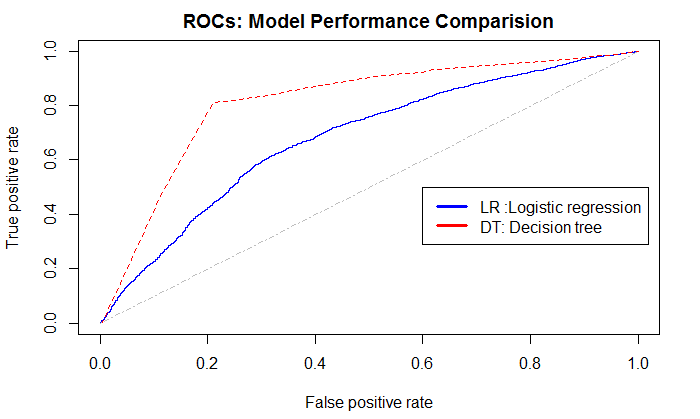
\includegraphics[width=\textwidth]{results1.png}
\centering
\caption{ROCs for logistic regression vs decision tree}{\textbf{Source:} Plotted in R Studio}
\label{fig:result}
\end{figure}
\end{center}

In table. \ref{table:results}, KS is the Kolmogorov-Smirnov goodness-of-Fit Test (or KS-Test), GINI is Gini coefficient of inequality distribution of response variable and AUC is Area under ROC (Receiver Operating Chaterstics) curve.


Receiver under curve is one of technique to estimate the performance of predictive model.

Limitations of data in real life application. Accuracy might vary

As provided was made up due to confidential agreement. Data is generated from pre-defined formulas which made it look quite original but it could cover all possible scenarios of real life. For example, it failed to consider a scenario when a customer is defaulting while being in creting rating 1 (Good Credit). \\

Intially, Logistic Regression and Decsion tree were giving accuracy of 99.31\% which is practially not possible in credit scoring. during this research work we found that various other researchers also pointed out that Logistic regression is much better modelling technique than any other statsical techqnique. For Instance Mr.x noted in work that neural network can work at par with logistic regression model provided that the target variable is predict result in yes or no.\\

Similarly decision tree has other limitations with respect to number of possible nodes and leafs for making creteria. hence decision tree end with less number of rules. Mr. Y compared the performance of Decesion tree and LR and found LR performance is higher than 5\%

As per dasssssssssssh paper 25 - 30\% error is expected in credit rating system because human nature is quite difficult to predict. Similar in this scenario it is quite complex to various parameter to consider to build solid system which have high accuracy. One of the leading bank in Ireland in past attempted to consider upto 600 parameter to all possible cases of credit using Artificial Intelligence 
testiing of model.

Accuracy reduced to 25\% after scaling variables. Compare difference between model performance and how it is improved.

How we implemented the model

Explaing Limitations of Algorithm and why one algo is better
FUTURE SCOPE IS AI of this credit scoring



%   MSc Business Analytics Dissertation
%
%   Title:     Aaa Bbbbbbb Cccccccccc
%   Author(s): Xxxxxx Xxxxxxxxx and Yyy Yyyyyyyyy
%
%   Chapter 6: Discussion
%
%   Change Control:
%   When     Who   Ver  What
%   -------  ----  ---  --------------------------------------------------------------
%   11Feb11  AB    0.1  Begun 
%

\chapter{Discussion}\label{C.Discussion}

\section{Introduction}\label{S.Discussion.intro}

In this chapter we examine \ldots

%   MSc Business Analytics Dissertation
%
%   Title:     Aaa Bbbbbbb Cccccccccc
%   Author(s): Xxxxxx Xxxxxxxxx and Yyy Yyyyyyyyy
%
%   Chapter 7: Conclusions and Future Research
%
%   Change Control:
%   When     Who   Ver  What
%   -------  ----  ---  --------------------------------------------------------------
%   11Feb11  AB    0.1  Begun 
%

\chapter{Conclusions and Future Research}\label{C.Conclusions.Future.research}

\begin{quote}
\textit{-- That's a most foolhardy remark, he said sharply, because the nerve-strings and 
the sheep's head itself are whirling into the same bargain and you can cancel out one whirl 
against the other and there you are --- like simplifying a division sum when you have fives 
above and below the bar.}

\textit{-- To say the truth I did not think of that.} 

\textit{-- Mollycules is a very intricate theorem and can be worked out with algebra but you 
would want to take it by degrees with rulers and cosines and familiar other instruments and 
then at the wind-up not believe what you had proved at all.  If that happened you would have 
to go over it till you got a place where you could believe your own facts and figures as 
exactly delineated from Hall and Knight's Algebra and then go on again from that particular 
place till you had the whole pancake properly believed and not have bits of it half-believed 
or a doubt in your head hurting you like when you lose the stud of your shirt in the middle 
of the bed.} 

\hspace{2cm}--- Flann O'Brien, \emph{The Dalkey Archive}
\end{quote}


\section{Introduction}\label{S.Concl.intro}

The significance of \ldots



%%   These next two items are more or less the same (epilogue is just the Greek for afterword!)
%%   They are unlikely to be long enough to justify their own file(s) to \include

%%   Epilogue (if any)
%%   Afterword (if any)

%% Back matter (loose ends: continue arabic page numbering)
\backmatter

%%   Appendices, if any: there will almost certainly be one or more.
%%   This is where you put material which the reader may like to refer to but which might break
%%   the train of thought in the thesis proper.  Large tables, etc might go here.
%%   You may also include program code if not too long: say a few important chunks.  But the
%%   majority of this should just be put on the accompanying CD/DVD.
%%   \include appendix/ces as it/they will be big enough to justify its/their own ``chapter(s)''
\cleardoublepage
\appendix
\addappheadtotoc         % adds a separating entry to the TOC, saying Appendices
\noappendicestocpagenum  % ensures there is no page number after that TOC separating entry
% It may happen that the first appendix (e.g., Detailed Tables) appears before the "Appendices" line
% in the table of contents.  If so, edit thesis.toc and move the Appendices line there above the first appendix,
% then re-run LaTeX to get the thesis.dvi file right.  You may have to repeatedly do this every time you LaTeX!
\cleardoublepage
%   MSc Business Analytics Dissertation
%
%   Title:     Aaa Bbbbbbb Cccccccccc
%   Author(s): Xxxxxx Xxxxxxxxx and Yyy Yyyyyyyyy
%
%   Appendix 1: long tables
%
%   Change Control:
%   When     Who   Ver  What
%   -------  ----  ---  --------------------------------------------------------------
%   11Feb11  AB    0.1  Begun 
%

\chapter{Detailed tables}\label{C.Appendix1}

Xyz

%   MSc Business Analytics Dissertation
%
%   Title:     Aaa Bbbbbbb Cccccccccc
%   Author(s): Xxxxxx Xxxxxxxxx and Yyy Yyyyyyyyy
%
%   Appendix 2: program code
%
%   Change Control:
%   When     Who   Ver  What
%   -------  ----  ---  --------------------------------------------------------------
%   11Feb11  AB    0.1  Begun 
%

\chapter{Program code}\label{C.Appendix2}

Xyz etc

% and so on

%%   Endnotes (if needed)

%%   Glossary of terms
%%   \include this as it may be big enough to justify its own ``chapter''
\cleardoublepage
\addcontentsline{toc}{chapter}{Glossary}
%   MSc Business Analytics Dissertation
%
%   Title:     Aaa Bbbbbbb Cccccccccc
%   Author(s): Xxxxxx Xxxxxxxxx and Yyy Yyyyyyyyy
%
%   Glossary
%
%   Change Control:
%   When     Who   Ver  What
%   -------  ----  ---  --------------------------------------------------------------
%   11Feb11  AB    0.1  Begun 
%

\chapter*{Glossary}\label{C.Glossary}

Entries are listed in alphabetical order.  



%%   Bibliography (References)
% For this, use BibTeX (invariably comes with your LaTeX installation).  BibTeX separates the form of a
% reference from its content, just as LaTeX does for a document.  You put the content in a .bib file
% called a BibTeX database, and tell BibTeX what style to overlay on it.
\cleardoublepage
\addcontentsline{toc}{chapter}{Bibliography}
\bibliographystyle{mscBA} % the BibTeX style file to use (omit the .bst suffix)
\bibliography{thesis}     % the BibTeX database file to use (omit the .bib suffix)
%
%% In the above, mscBA.bst is a BibTeX style file I developed based on the fairly standard chicago.bst.
%%
%% Below are sample journal and book entries from a .bib file.  Ensure that the key e.g., Chomsky:1965 you use
%% in your .bib file entry is the same as you use in the \cite{Chomsky:1965} command in your LaTeX file.
%%
%% @String{MIT = {{MIT Press}}}
%% @String{MIT:adr = {{Cambridge, Massachusetts}}}
%%
%% @Article{MetropEtAl:1953,
%%  AUTHOR =       {Metropolis, N. and A.W. Rosenbluth and M.N. Rosenbluth and A.H. Teller and E. Teller},
%%  YEAR =         {1953},
%%  TITLE =        {Equations of {S}tate Calculations by Fast Computing Machines},
%%  JOURNAL =      {Journal of Chemical Physics},
%%  VOLUME =       {21},
%%  NUMBER =       {6},
%%  PAGES =        {1087--1092}
%% }
%%
%% @Book{Chomsky:1965,
%%   Author =       {N. Chomsky},
%%   title =        {Aspects of the theory of syntax},
%%   PUBLISHER =    MIT,
%%   ADDRESS =      MIT:adr,
%%   YEAR =         1965
%% }
%%
%% Some other points (see the sample bibfile entries above for illustration):
%% - Case is unimportant for a field name: DATE, daTe and date all mean the same.
%% - You separate multiple authors by 'and', not using commas etc.
%% - Some punctuation marks in the key are OK, e.g. the colon ':' as in MetropEtAl:1953
%% - BibTeX has its own internal rules on when to change the case of capitalised text (e.g. in journal article titles).
%%   You can override this by putting braces {} around text you want unchanged (e.g. the S in the article title above.
%% - You can define strings which will be expanded in the references, e.g., MIT and MIT:adr in the book above
%%   Don't put braces or quotes around these: if you do, they will not be expanded (will remain as MIT:adr, say)
%% - In your actual text, you can cite in two ways (note the position of parentheses):
%%   \citep{MetropEtAl:1953} for citation in parentheses, e.g.,
%%     "In \citep{MetropEtAl:1953} it is shown that ..." appears as "In (Metropolis et al, 1953) it is shown that ..."
%%   \citet{MetropEtAl:1953} for citation in text, e.g., where the authors are the subject of the sentence:
%%     "\citet{MetropEtAl:1953} show that ..." appears as "Metropolis et al (1953) show that ..."
%% - With either \citep or \citet you can use optional arguments such as
%%     "\citep[e.g.,][pp.~12--20]{MetropEtAl:1953}" appears as "(e.g., Metropolis et al, 1953, pp.~12--20)"

%%   List of contributors -- anyone else you feel should be credited

%%   Notation Index / List of Symbols
%%   \include this as it may be big enough to justify its own ``chapter''
\cleardoublepage
\addcontentsline{toc}{chapter}{List of Notation}
%   MSc Business Analytics Dissertation
%
%   Title:     Aaa Bbbbbbb Cccccccccc
%   Author(s): Xxxxxx Xxxxxxxxx and Yyy Yyyyyyyyy
%
%   List of Notation
%
%   Change Control:
%   When     Who   Ver  What
%   -------  ----  ---  --------------------------------------------------------------
%   11Feb11  AB    0.1  Begun 
%

\chapter*{List of Notation}\label{C.Notation}

Entries are listed in the order of appearance.  The ``Ref'' is the number of the section, 
definition, etc., in which the notation is explained.

\vspace{0.5cm}

{\renewcommand{\arraystretch}{0.9}

\begin{tabular}{llr}
\tb{Symbol}  & \tb{Description} & \tb{Ref}   \\\hline
$\FF_q $  & Finite field of $q$ elements & \ref{Th.FF.fte.field}  \\
\end{tabular}


}



%%   Index
\cleardoublepage
\addcontentsline{toc}{chapter}{Index}
\printindex

\end{document}
